% !TEX root = ../main_v2.tex
\section{Numerical Validation}
\label{sec:numerical_results}

The exact solution of Sec.~\ref{sec:qubit_direct_response_v5} depends on the
bath only through the kernel evaluated at three frequencies,
$\omega \in \{0, \pm\omega_q\}$.
To test it we compare against Exact Diagonalisation (ED) of a truncated
spin-boson model: the qubit is coupled to $N_\omega$ harmonic oscillators,
each represented with a per-mode Fock cutoff $n_{\max}$.
A key feature of this comparison is that the analytic kernel integrals
$\mathcal{K}(\omega) = \int_0^\infty d\nu\, J(\nu)\, \mathcal{F}(\nu,\omega,\beta)$
can be evaluated in two ways: using the full continuum spectral density
(the \emph{continuous analytic} branch) or restricted to the same $N_\omega$
discrete modes seen by ED (the \emph{discrete analytic} branch).
Distinguishing between these is essential for identifying the true origin 
of numerical discrepancies in the strong-coupling regime.

\subsection*{The representability bottleneck: Fig.~\protect\ref{fig:ed_vs_analytic}}

Figure~\ref{fig:ed_vs_analytic} shows the excited-state population $p_{11}$
as a function of coupling strength (panel~a, $\beta\omega_q = 2$,
$\theta = \pi/4$) and inverse temperature (panel~b, $g/\omega_q = 0.5$,
$\theta = \pi/2$), each for $N_\omega = 40$ modes.
At weak coupling ($\chi \ll 1$) all three curves coincide.
However, as the system crosses into the strong-coupling regime ($\chi \gtrsim 1$),
the continuous analytic prediction separates from the ED results.

The key to interpreting this gap lies in the \emph{discrete analytic} branch
(blue dashed line). This branch evaluates the HMF formula on the exact
discrete spectral density of the simulation. Crucially, as $\chi$ increases,
the discrete analytic result does not follow the ED curve; instead, it
tracks the continuous analytic branch and correctly converges to the
ultrastrong fixed point. This is a powerful result: it shows that the HMF
theory is exact even for small, discrete mode sets, and that a discrete 
bath is physically capable of reaching the ultrastrong limit.

The fact that ED (green solid) remains significantly higher than its own
infinite-cutoff analytic prediction is therefore not a failure of the theory,
nor even a finite-bath artifact. Rather, it is a **representability bottleneck**.
In the ultrastrong limit, the coupled system seeks a displaced ground state
(a polaron-like state) where each mode $k$ is displaced from vacuum by
$\alpha_k \sim g_k/\omega_k$. Representing such a state faithfully requires
a Fock cutoff $n_{\max} \gtrsim |\alpha_k|^2$. When $\chi \gtrsim 1$, the
available Fock space in the ED simulation is insufficient to capture the
tails of these displaced oscillators. The system is "trapped" in a subspace
of artificially low occupation numbers, leading to over-estimated energies
and the persistent gap observed at large $\chi$ and low $T$.

\begin{figure}[t]
  \centering
  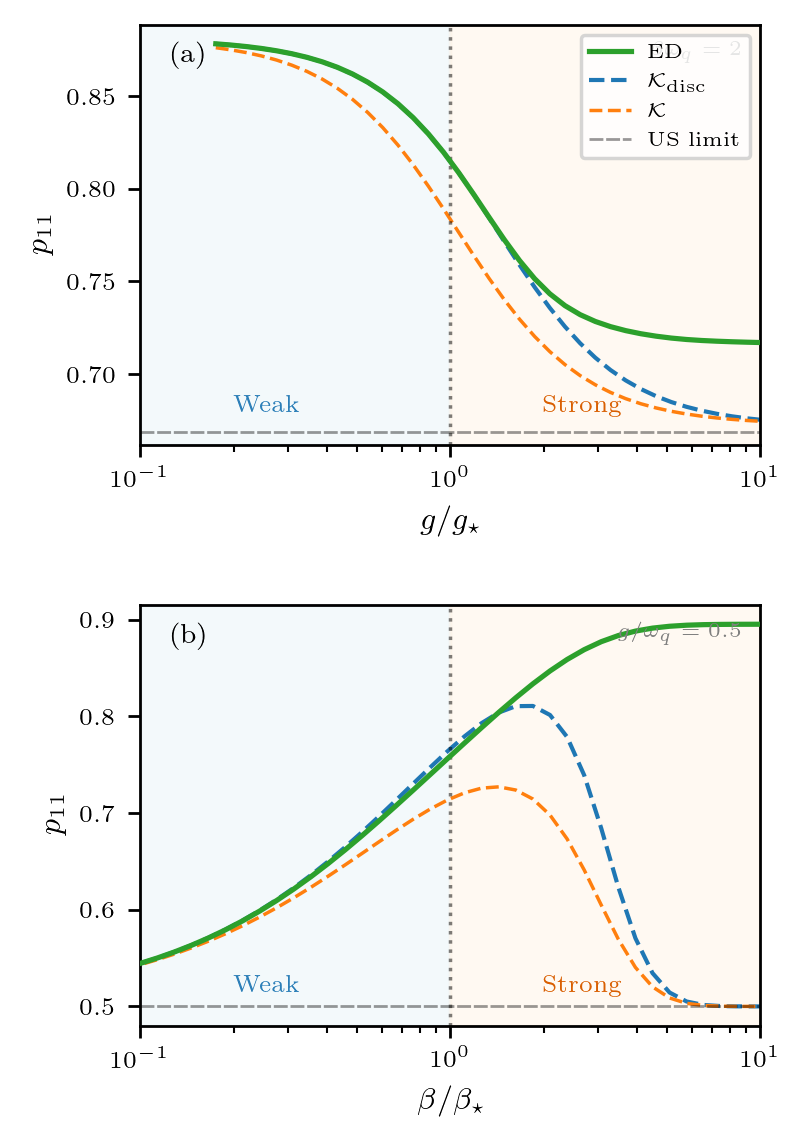
\includegraphics[width=0.48\textwidth]{../figures/hmf_fig2_ed_vs_analytic.png}
  \caption{Excited-state population $p_{11}$ across the $\chi$-crossover
    for $N_\omega=40$ modes.
    Green solid: ED.  Blue dashed: discrete analytic (same $N_\omega$ modes).
    Orange dotted: continuous analytic.
    Dashed horizontal lines mark the ultrastrong limit $p_\infty$.
    The discrete analytic correctly reaches the US limit, 
    matching the continuum. The gap left by ED (green) is a representability 
    failure: the fixed Fock cutoff cannot accommodate the mode displacements 
    required to reach the true HMF state.}
  \label{fig:ed_vs_analytic}
\end{figure}

\subsection*{Simulability as a mode-occupation problem: Fig.~\protect\ref{fig:bandwidth_convergence}}

If the bottleneck is indeed a representability limit on mode occupancy, the 
performance of the numerical simulation should be highly sensitive to how 
the spectral weight is distributed among individual modes. 
Figure~\ref{fig:bandwidth_convergence} explores this by varying the 
spectral window bandwidth $B$ for a small three-mode bath ($N_\omega = 3$).

Panel~(a) shows that the RMSE between ED and the analytic prediction is 
non-monotone, with a sharp increase beyond the "magic bandwidth" $B^* = 3.8$.
The interpretation from Fig.~\ref{fig:ed_vs_analytic} makes this failure 
inevitable: increasing $B$ for fixed $N_\omega$ moves modes away from 
resonance into the high-frequency tail. While these off-resonant modes have 
smaller individual couplings $g_k$, the total displacement "load" they carry 
collectively in the US limit remains high. At low temperatures (high $\chi$), 
this load forces the simulation into the representability bottleneck.

This is confirmed in Panel~(b), where the cutoff sensitivity 
(the difference between $n_{\max}=4$ and $n_{\max}=6$) peaks exactly in the 
region where $B \approx B^*$. This peak is a direct signature of the modes 
"hitting" the Fock cutoff as they attempt to polarize. The effect is 
maximal at low temperature, where the $\chi$-driven displacement requirements 
are most severe. Finally, Panel~(c) show that for a fixed "optimal" 
bandwidth $B_{\mathrm{opt}}$, the simulation remains converged at high $T$ 
($\chi \ll 1$) but uniformly fails as $\beta \to \infty$ ($\chi \gg 1$), 
with the curves for different $n_{\max}$ branching off at the crossover scale.
Simulation success is thus not a matter of bandwidth per se, but of whether 
the discrete bath's occupancy requirements exceed the representable 
Hilbert space.

\begin{figure*}[t]
  \centering
  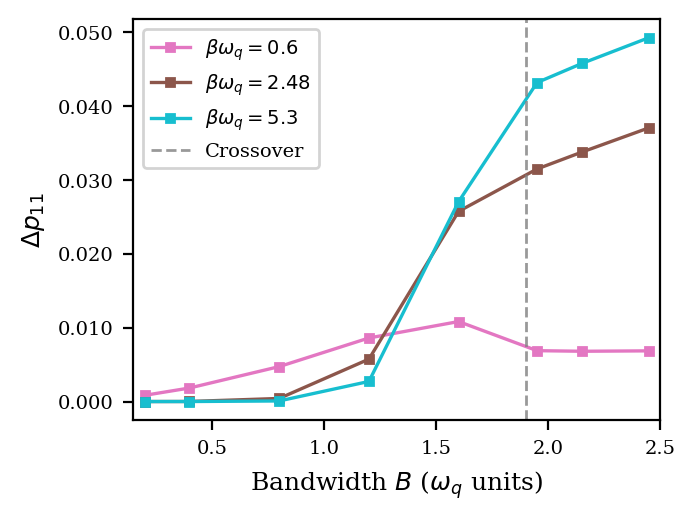
\includegraphics[width=0.95\textwidth]{../figures/hmf_fig3_bandwidth_convergence.png}
  \caption{Representability and simulability for $N_\omega = 3$.
    \textit{Panel~(a)}: Averaged RMSE versus bandwidth; the error rises past
    the magic bandwidth $B^*$.
    \textit{Panel~(b)}: Cutoff sensitivity peaks at low temperature ($\chi > 1$)
    around $B \approx B^*$.
    \textit{Panel~(c)}: Absolute residual grows and branches as a function
    of inverse temperature, with the representability bottleneck appearing
    exactly at the $\chi \sim 1$ crossover.}
  \label{fig:bandwidth_convergence}
\end{figure*}

In summary, the numerical results establish that the analytic HMF provides 
the correct physical target for both discrete and continuous baths. The 
deviations seen in simulation are not theoretical errors but markers of the 
intrinsic difficulty in representing the strongly-dressed open-system ground 
state within a finite Fock basis. The crossover parameter $\chi$ emerges as 
the universal controller of this "simulability" crossover, just as it 
governs the analytic structure of the state itself.
